\documentclass{standalone}
\usepackage{tikz}
\usetikzlibrary{patterns}
\usetikzlibrary{positioning}
\usetikzlibrary{patterns, positioning}
\usetikzlibrary{shapes.misc}
\usepackage[outline]{contour}
\contourlength{1.5pt} 
\usepackage[sfdefault]{ClearSans}

\begin{document}
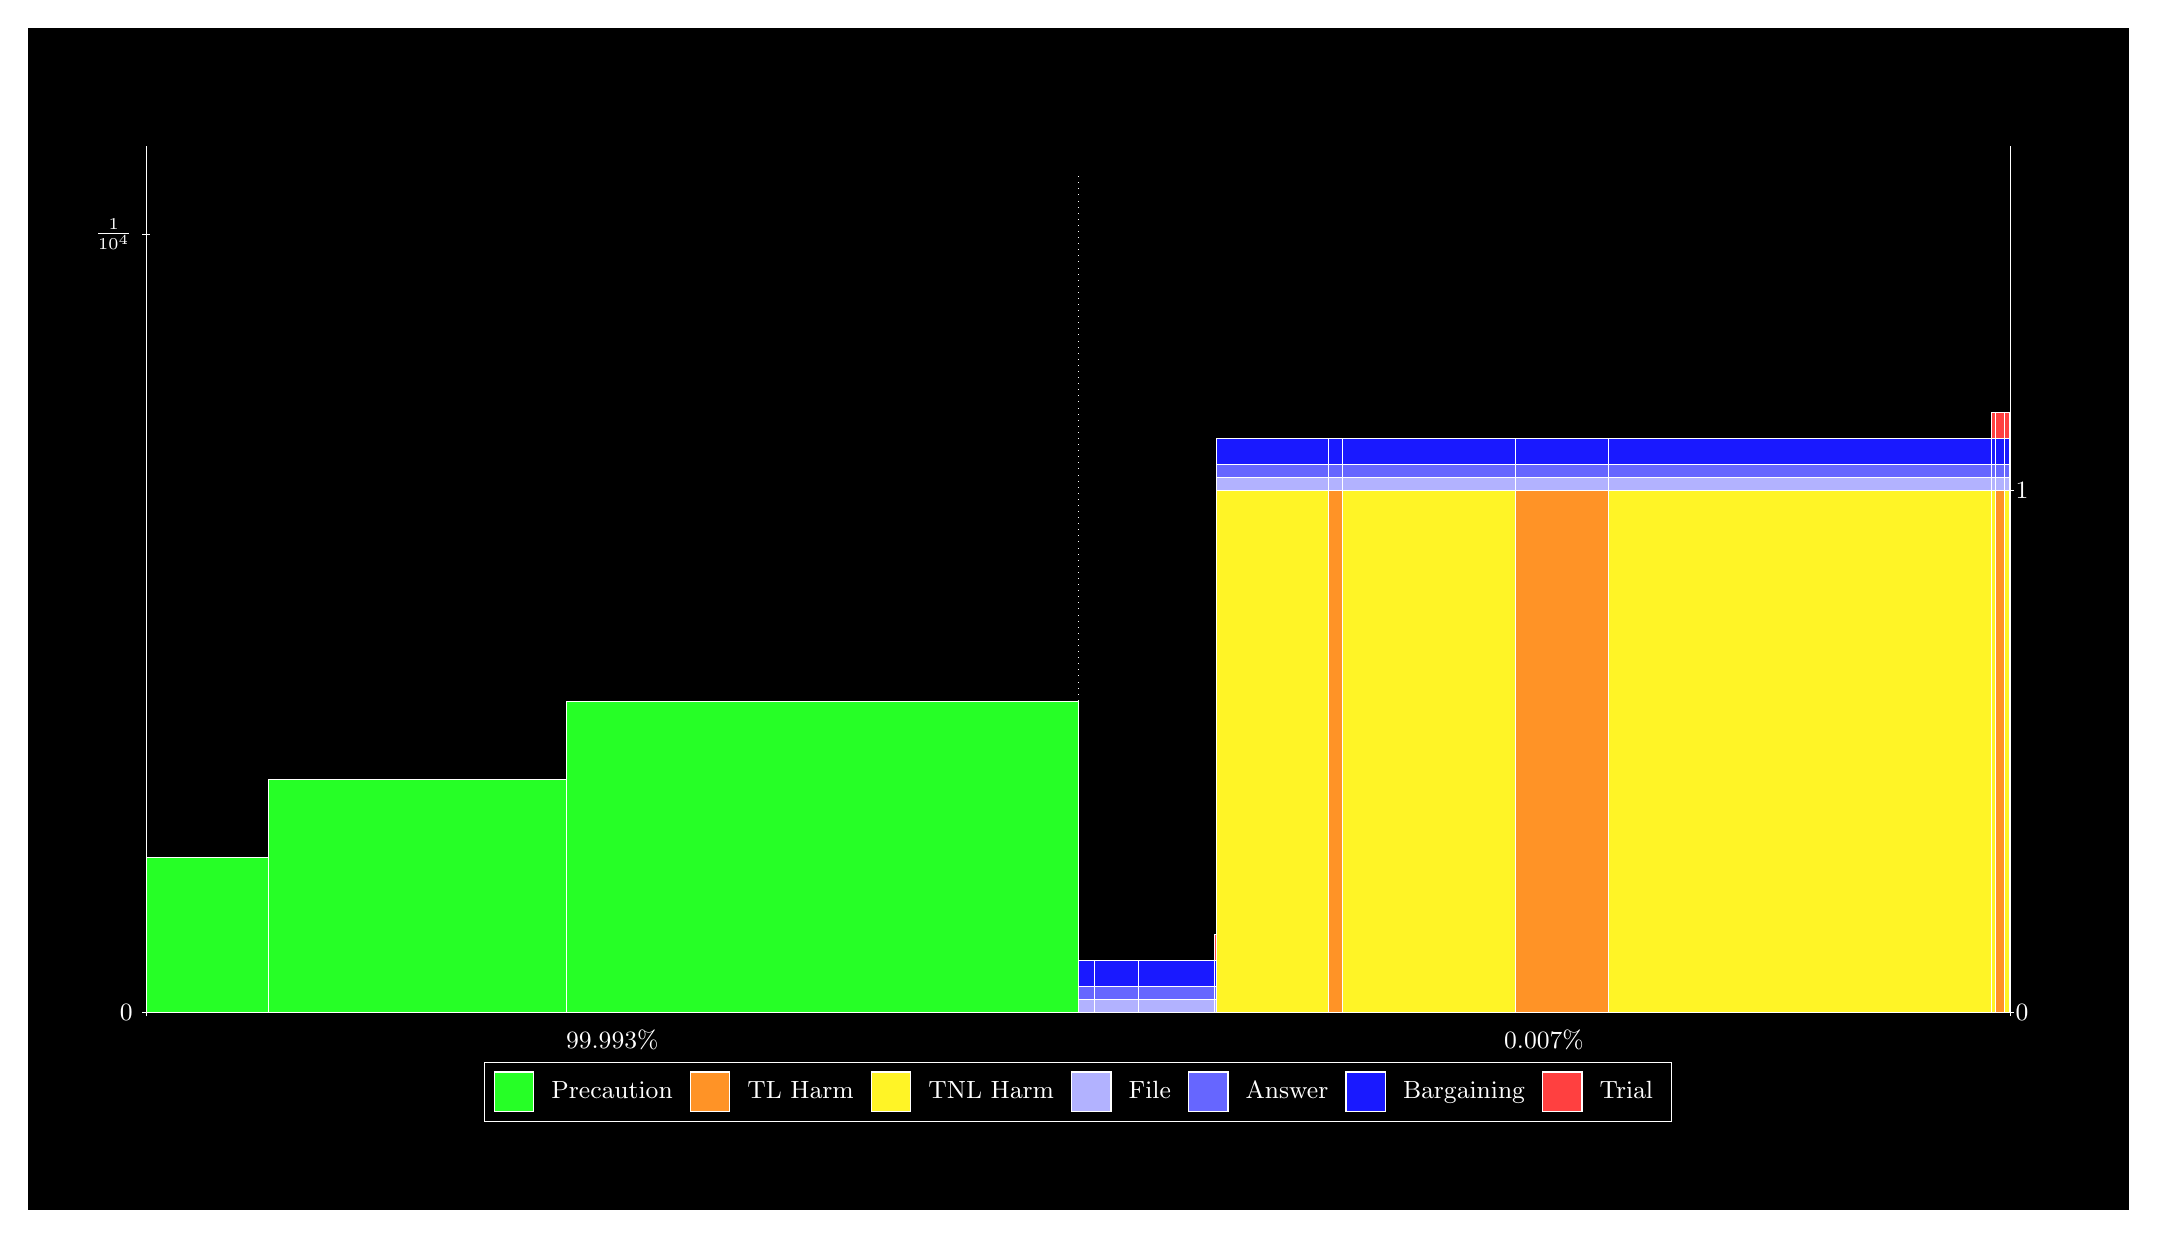
\begin{tikzpicture}
\draw[fill=black] (0,0) rectangle (26.667,15);
\draw[fill=green!85,draw=white,very thin] (1.5,2.5) rectangle (3.0457,4.4771);
\draw[fill=green!85,draw=white,very thin] (3.0457,2.5) rectangle (6.8344,5.4656);
\draw[fill=green!85,draw=white,very thin] (6.8344,2.5) rectangle (13.333,6.4541);
\draw[fill=green!85,draw=white,very thin] (13.333,2.5) rectangle (13.539,2.5001);
\draw[fill=blue!30,draw=white,very thin] (13.333,2.5001) rectangle (13.539,2.666);
\draw[fill=blue!60,draw=white,very thin] (13.333,2.666) rectangle (13.539,2.8318);
\draw[fill=blue!90,draw=white,very thin] (13.333,2.8318) rectangle (13.539,3.1634);
\draw[fill=green!85,draw=white,very thin] (13.539,2.5) rectangle (14.093,2.5002);
\draw[fill=blue!30,draw=white,very thin] (13.539,2.5002) rectangle (14.093,2.666);
\draw[fill=blue!60,draw=white,very thin] (13.539,2.666) rectangle (14.093,2.8319);
\draw[fill=blue!90,draw=white,very thin] (13.539,2.8319) rectangle (14.093,3.1635);
\draw[fill=green!85,draw=white,very thin] (14.093,2.5) rectangle (15.062,2.5003);
\draw[fill=blue!30,draw=white,very thin] (14.093,2.5003) rectangle (15.062,2.6661);
\draw[fill=blue!60,draw=white,very thin] (14.093,2.6661) rectangle (15.062,2.8319);
\draw[fill=blue!90,draw=white,very thin] (14.093,2.8319) rectangle (15.062,3.1636);
\draw[fill=green!85,draw=white,very thin] (15.062,2.5) rectangle (15.086,2.5001);
\draw[fill=blue!30,draw=white,very thin] (15.062,2.5001) rectangle (15.086,2.666);
\draw[fill=blue!60,draw=white,very thin] (15.062,2.666) rectangle (15.086,2.8318);
\draw[fill=blue!90,draw=white,very thin] (15.062,2.8318) rectangle (15.086,3.1634);
\draw[fill=red!75,draw=white,very thin] (15.062,3.1634) rectangle (15.086,3.4951);
\draw[fill=green!85,draw=white,very thin] (15.086,2.5) rectangle (16.51,2.5001);
\draw[fill=yellow!85,draw=white,very thin] (15.086,2.5001) rectangle (16.51,9.1333);
\draw[fill=blue!30,draw=white,very thin] (15.086,9.1333) rectangle (16.51,9.2991);
\draw[fill=blue!60,draw=white,very thin] (15.086,9.2991) rectangle (16.51,9.4649);
\draw[fill=blue!90,draw=white,very thin] (15.086,9.4649) rectangle (16.51,9.7966);
\draw[fill=green!85,draw=white,very thin] (16.51,2.5) rectangle (16.689,2.5001);
\draw[fill=orange!85,draw=white,very thin] (16.51,2.5001) rectangle (16.689,9.1333);
\draw[fill=blue!30,draw=white,very thin] (16.51,9.1333) rectangle (16.689,9.2991);
\draw[fill=blue!60,draw=white,very thin] (16.51,9.2991) rectangle (16.689,9.4649);
\draw[fill=blue!90,draw=white,very thin] (16.51,9.4649) rectangle (16.689,9.7966);
\draw[fill=green!85,draw=white,very thin] (16.689,2.5) rectangle (18.885,2.5002);
\draw[fill=yellow!85,draw=white,very thin] (16.689,2.5002) rectangle (18.885,9.1333);
\draw[fill=blue!30,draw=white,very thin] (16.689,9.1333) rectangle (18.885,9.2992);
\draw[fill=blue!60,draw=white,very thin] (16.689,9.2992) rectangle (18.885,9.465);
\draw[fill=blue!90,draw=white,very thin] (16.689,9.465) rectangle (18.885,9.7966);
\draw[fill=green!85,draw=white,very thin] (18.885,2.5) rectangle (20.061,2.5002);
\draw[fill=orange!85,draw=white,very thin] (18.885,2.5002) rectangle (20.061,9.1333);
\draw[fill=blue!30,draw=white,very thin] (18.885,9.1333) rectangle (20.061,9.2992);
\draw[fill=blue!60,draw=white,very thin] (18.885,9.2992) rectangle (20.061,9.465);
\draw[fill=blue!90,draw=white,very thin] (18.885,9.465) rectangle (20.061,9.7966);
\draw[fill=green!85,draw=white,very thin] (20.061,2.5) rectangle (24.926,2.5003);
\draw[fill=yellow!85,draw=white,very thin] (20.061,2.5003) rectangle (24.926,9.1334);
\draw[fill=blue!30,draw=white,very thin] (20.061,9.1334) rectangle (24.926,9.2992);
\draw[fill=blue!60,draw=white,very thin] (20.061,9.2992) rectangle (24.926,9.4651);
\draw[fill=blue!90,draw=white,very thin] (20.061,9.4651) rectangle (24.926,9.7967);
\draw[fill=green!85,draw=white,very thin] (24.926,2.5) rectangle (24.975,2.5001);
\draw[fill=yellow!85,draw=white,very thin] (24.926,2.5001) rectangle (24.975,9.1333);
\draw[fill=blue!30,draw=white,very thin] (24.926,9.1333) rectangle (24.975,9.2991);
\draw[fill=blue!60,draw=white,very thin] (24.926,9.2991) rectangle (24.975,9.4649);
\draw[fill=blue!90,draw=white,very thin] (24.926,9.4649) rectangle (24.975,9.7966);
\draw[fill=red!75,draw=white,very thin] (24.926,9.7966) rectangle (24.975,10.128);
\draw[fill=green!85,draw=white,very thin] (24.975,2.5) rectangle (25.096,2.5001);
\draw[fill=orange!85,draw=white,very thin] (24.975,2.5001) rectangle (25.096,9.1333);
\draw[fill=blue!30,draw=white,very thin] (24.975,9.1333) rectangle (25.096,9.2991);
\draw[fill=blue!60,draw=white,very thin] (24.975,9.2991) rectangle (25.096,9.4649);
\draw[fill=blue!90,draw=white,very thin] (24.975,9.4649) rectangle (25.096,9.7966);
\draw[fill=red!75,draw=white,very thin] (24.975,9.7966) rectangle (25.096,10.128);
\draw[fill=green!85,draw=white,very thin] (25.096,2.5) rectangle (25.161,2.5002);
\draw[fill=yellow!85,draw=white,very thin] (25.096,2.5002) rectangle (25.161,9.1333);
\draw[fill=blue!30,draw=white,very thin] (25.096,9.1333) rectangle (25.161,9.2992);
\draw[fill=blue!60,draw=white,very thin] (25.096,9.2992) rectangle (25.161,9.465);
\draw[fill=blue!90,draw=white,very thin] (25.096,9.465) rectangle (25.161,9.7966);
\draw[fill=red!75,draw=white,very thin] (25.096,9.7966) rectangle (25.161,10.128);
\draw[fill=green!85,draw=white,very thin] (25.161,2.5) rectangle (25.167,2.5002);
\draw[fill=orange!85,draw=white,very thin] (25.161,2.5002) rectangle (25.167,9.1333);
\draw[fill=blue!30,draw=white,very thin] (25.161,9.1333) rectangle (25.167,9.2992);
\draw[fill=blue!60,draw=white,very thin] (25.161,9.2992) rectangle (25.167,9.465);
\draw[fill=blue!90,draw=white,very thin] (25.161,9.465) rectangle (25.167,9.7966);
\draw[fill=red!75,draw=white,very thin] (25.161,9.7966) rectangle (25.167,10.128);
\draw[white,very thin] (1.5,2.5) -- (1.5,13.5);
\draw[white,very thin] (1.45,2.5) -- (1.55,2.5);
\node[font=\small,text=white, anchor=east] at (1.45, 2.5) {0};
\draw[white,very thin] (1.45,12.385) -- (1.55,12.385);
\node[font=\small,text=white, anchor=east] at (1.45, 12.385) {$\frac{1}{10^{4}}$};

\draw[white,dotted,very thin] (13.333,2.83) -- (13.333,13.17);
\draw[white,very thin] (25.167,2.5) -- (25.167,13.5);
\draw[white,very thin] (25.117,2.5) -- (25.217,2.5);
\node[font=\small,text=white, anchor=west] at (25.117, 2.5) {0};
\draw[white,very thin] (25.117,9.1331) -- (25.217,9.1331);
\node[font=\small,text=white, anchor=west] at (25.117, 9.1331) {1};

\draw[white,very thin] (1.5,2.5) -- (25.167,2.5);
\draw[white,very thin] (1.5,2.45) -- (1.5,2.55);
\node[font=\small,text=white, anchor=north] at (1.5, 2.45) {};
\draw[white,very thin] (25.167,2.45) -- (25.167,2.55);
\node[font=\small,text=white, anchor=north] at (25.167, 2.45) {};

\node[font=\small,text=white,anchor=south] at (7.4167, 1.9) {99.993\%};
\node[font=\small,text=white,anchor=south] at (19.25, 1.9) {0.007\%};
\draw (13.3333,2.5) node (B) {};
\begin{scope}[align=center]
\matrix[scale=0.5,draw=white,below=0.5cm of B,nodes={draw},column sep=0.1cm]{
\node[rectangle,draw,minimum width=0.5cm,minimum height=0.5cm,fill=green!85]{}; & \node[draw=none,font=\small,text=white]{Precaution}; &
\node[rectangle,draw,minimum width=0.5cm,minimum height=0.5cm,fill=orange!85]{}; & \node[draw=none,font=\small,text=white]{TL Harm}; &
\node[rectangle,draw,minimum width=0.5cm,minimum height=0.5cm,fill=yellow!85]{}; & \node[draw=none,font=\small,text=white]{TNL Harm}; &
\node[rectangle,draw,minimum width=0.5cm,minimum height=0.5cm,fill=blue!30]{}; & \node[draw=none,font=\small,text=white]{File}; &
\node[rectangle,draw,minimum width=0.5cm,minimum height=0.5cm,fill=blue!60]{}; & \node[draw=none,font=\small,text=white]{Answer}; &
\node[rectangle,draw,minimum width=0.5cm,minimum height=0.5cm,fill=blue!90]{}; & \node[draw=none,font=\small,text=white]{Bargaining}; &
\node[rectangle,draw,minimum width=0.5cm,minimum height=0.5cm,fill=red!75]{}; & \node[draw=none,font=\small,text=white]{Trial}; \\\\
};\end{scope}

\end{tikzpicture}
\end{document}